%!TEX root = ../main.tex
\section{3D mapping validated in simulation}
\label{sec:chap3}

The Aracati2017 dataset cannot evaluate a 3D map: the P900 provides a single
horizontal fan, and the ground truth contains no 3D model of the marina. We
therefore validate the 3D extension in the \textbf{HoloOcean} simulator~\hyperref[bib:holoocean]{[11]},
which provides both the additional sonars and an exact reference. The principle
of this chapter is deliberately simple: \textbf{the SLAM chain of chapter~2 is
kept unchanged, and only the point cloud becomes 3D} — two extra sonars observe
the vertical dimension, and their returns are placed along the trajectory
estimated by the 2D SLAM.

\subsection{Simulation setup}
\label{sec:holo-setup}

The scene is the \emph{PierHarbor} environment: two docks standing on piles,
about 50~m apart, with a floating vessel (draught 2.9~m) moored along the west
dock. The vehicle carries three acoustic sensors and a navigation suite
(\autoref{tab:holo-sensors}); all measurements are published in the vehicle
frame, and the simulator ground truth is recorded for \textbf{evaluation only},
so the GT-free rule of the introduction applies unchanged.

\begin{figure}[H]
\centering
\fbox{\parbox[c][4.2cm][c]{0.75\textwidth}{\centering
(vehicle and sensor layout — hand drawing to be added)}}
\caption{Vehicle and sensor layout: horizontal SLAM sonar and vertical fan
looking forward (the ``+''), transverse 360° profiler, DVL/IMU/depth.}
\label{fig:holo-uv}
\end{figure}

\begin{table}[H]
\centering
\small
\begin{tabular}{llcccc}
\hline
Sensor & Mount & Coverage & Range & Image & Rate \\
\hline
Imaging sonar (SLAM) & horizontal, forward & 120° azimuth & 0.5--20 m & 1024$\times$512 & 5 Hz \\
Imaging sonar (3D)   & rolled 90°, forward & 120° elevation & 0.5--20 m & 512$\times$256 & 5 Hz \\
Profiling sonar      & transverse ring     & 360°           & 0.5--20 m & 512$\times$720 & 2 Hz \\
DVL                  & down                & --             & --        & $\sigma$ 0.01 m/s & 5 Hz \\
IMU                  & --                  & --             & --        & $\sigma_g$ 0.002 rad/s & 50 Hz \\
Depth                & --                  & --             & --        & $\sigma$ 0.02 m & 5 Hz \\
\hline
\end{tabular}
\caption{Sensor suite. The 3D sonar is the same model as the SLAM sonar,
mounted 0.15~m above it; the profiling sonar scans a vertical ring
perpendicular to the direction of travel (0.5°/beam).}
\label{tab:holo-sensors}
\end{table}

The odometry is a dead-reckoning node that integrates the IMU orientation and
the DVL body velocities. The default simulated sensors are nearly perfect
(drift of 0.14~m over 24~min), which would make any SLAM evaluation
meaningless; we therefore inject a realistic error model into the sensor
streams before they reach the pipeline:
\begin{itemize}
\item compass: 1° constant bias plus a random walk of 0.05°/$\sqrt{\text{s}}$
  ($\approx$1.9° standard deviation at the end of the run), typical of a
  magnetic compass near steel structures;
\item DVL: $+0.3\,\%$ scale error and 0.5° mount misalignment, typical
  manufacturer figures;
\item white noise on all channels (gyro, accelerometer, DVL, depth) with the
  standard deviations of \autoref{tab:holo-sensors}.
\end{itemize}
The vehicle follows an analytic path (positions imposed at each tick, no
hydrodynamic model): a single lap of \textbf{443~m in 23~min} (0.35~m/s) around
the rectangle formed by the two docks, at constant depth $-6.5$~m — which makes
the vehicle pass \emph{under} the moored vessel with 3.6~m of clearance.

\subsection{Two extra sonars: the ``+'' configuration}
\label{sec:holo-plus}

A forward-looking sonar measures range and azimuth but not elevation: every
echo inside its vertical aperture is flattened onto the image plane. The 2D
SLAM tolerates this ambiguity, but a 3D map cannot be built from it. Following
the orthogonal-pair idea of McConnell et al.~\hyperref[bib:mcconnell]{[12]}, we add a second, identical
imaging sonar rolled by 90°: its fan is vertical, so it resolves elevation
exactly where the SLAM sonar resolves azimuth (a ``+'' seen from the front).
The transverse profiling sonar completes the coverage with a full vertical
section (seabed and both sides) every 17.5~cm of travel.

The 3D map is then built \textbf{offline}, without touching the SLAM:
\begin{itemize}
\item each ping of the vertical fan and of the profiler keeps, per beam, the
  strongest return (one wall per beam), expressed in the vehicle frame;
\item these points are placed along the SLAM trajectory: $(x, y, \theta)$ from
  the 2D pose graph, $z$ from the depth sensor;
\item two filters remove the known artefacts: echoes of the water surface, and
  out-of-plane ghosts of the wide-aperture fans; the cloud is finally
  decimated on a 0.2~m voxel grid.
\end{itemize}

\subsection{Results}
\label{sec:holo-results}

\autoref{tab:holo-results} summarises the run. Since the simulator ground
truth is exact and complete, we report the standard Umeyama-aligned
ATE~\hyperref[bib:umeyama]{[7]} here (the start-pinned protocol of \autoref{sec:protocole} was designed
for the position-only DGPS of Aracati); the map is compared with the reference
cloud obtained by placing the \emph{same} sonar returns along the ground-truth
trajectory.

\begin{table}[H]
\centering
\small
\begin{tabular}{lc}
\hline
Keyframes & 837 \\
ATE (Umeyama) & \textbf{1.14 m} (0.26\,\% of the 443 m path) \\
Heading error & median 0.7°, RMS 1.1° \\
3D map & 155\,284 points (0.2 m voxel) \\
Map vs reference cloud & NN median \textbf{0.218 m}, p90 1.69 m \\
\hline
\end{tabular}
\caption{Proposed method (chapter~2) on the simulated one-lap mission.}
\label{tab:holo-results}
\end{table}

One point must be stated plainly: on this run the loop-closure stage accepts
\textbf{no candidate}, and the estimate coincides with dead reckoning (maximum
difference below 0.1~mm). With the error model above, the odometry drifts by
about 1~m over the lap — there is simply nothing left for the loops to correct.
The numbers of \autoref{tab:holo-results} therefore validate the
\textbf{3D mapping chain} (mounts, reprojection, filters) rather than the loop
closures, which chapter~2 already evaluated on real data.

\begin{figure}[H]
\centering
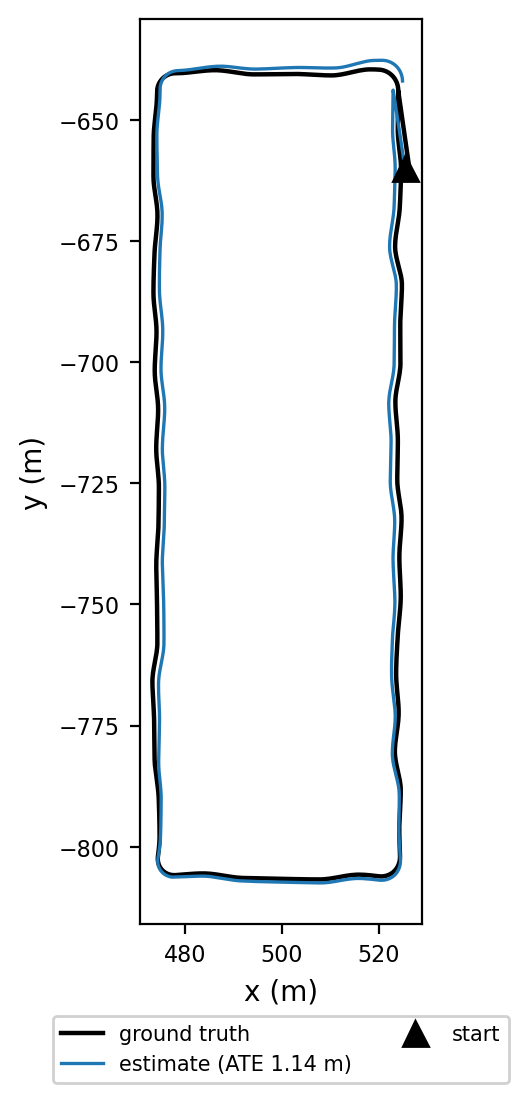
\includegraphics[width=0.42\textwidth]{Image/Holo_traj_BS9.png}
\caption{Estimated trajectory against ground truth (Umeyama alignment). The
lap is 443 m long; the final ATE is 1.14 m.}
\label{fig:holo-traj}
\end{figure}

\autoref{fig:holo-carte} shows the resulting map, drawn with the real
proportions of the scene (198$\times$98$\times$22 m). One recognises the two
rows of dock piles, the hull of the moored vessel above the west leg of the
trajectory, and the seabed swept by the profiler. The median distance to the
reference cloud is 0.218~m — about the voxel size; the 90\textsuperscript{th}
percentile (1.69~m) is dominated by the sparse echoes at the edges of the
sonar coverage.

\begin{figure}[H]
\centering
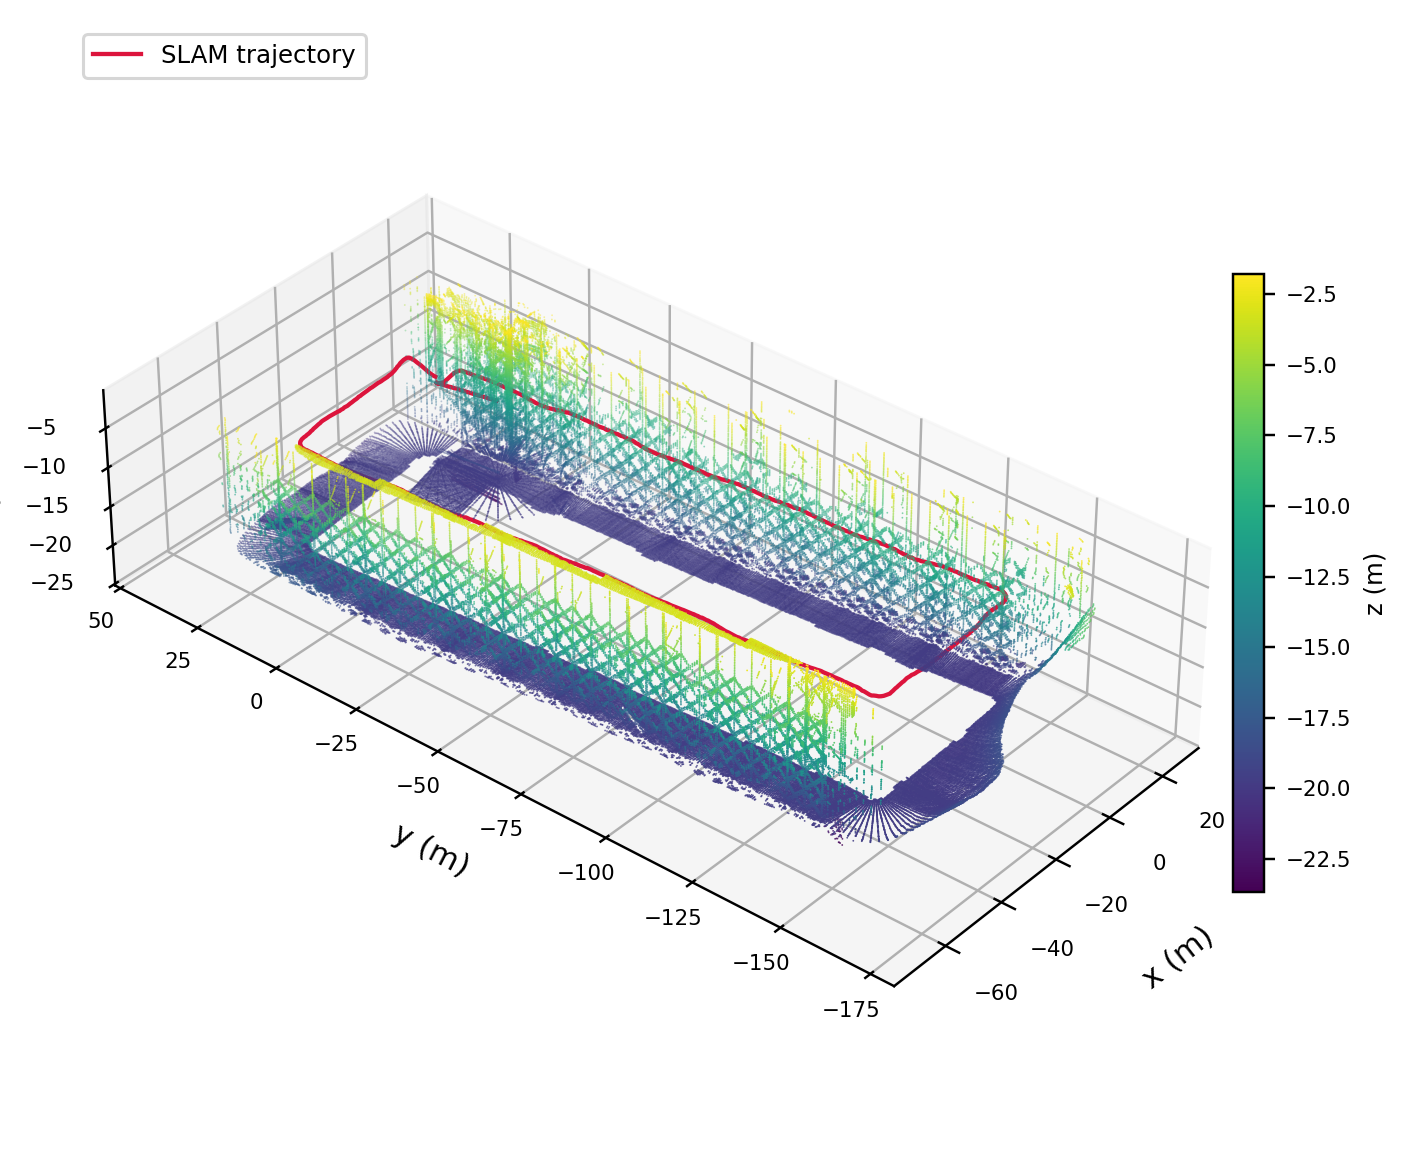
\includegraphics[width=\textwidth]{Image/Holo_carte3d_BS9.png}
\caption{GT-free 3D map (155\,284 points, coloured by depth) and SLAM
trajectory (red). Dock piles, vessel hull and seabed are all obtained from
the embedded sensors only.}
\label{fig:holo-carte}
\end{figure}

\subsection{Limits}
\label{sec:holo-limits}

\begin{itemize}
\item The simulated sonar images are cleaner than real ones (no multipath, no
  reverberation): the feature extraction works in easier conditions than in
  chapters~1--2.
\item HoloOcean provides no USBL sensor, so the anchoring of chapter~1 is not
  exercised here.
\item The vehicle is moved analytically (no hydrodynamic model), and a single
  run per configuration is reported.
\end{itemize}

Conclusion: with the base pipeline kept unchanged, two additional sonars and an
offline reprojection are enough to turn the 2D SLAM into a usable 3D map, at
0.22~m median error from the reference in a 200~m-scale harbour scene.
